%----------------------------------------------------------------
%
%  File    :  thesis.tex
%
%  Authors :  Keith Andrews, IICM, TU Graz, Austria
%             Manuel Koschuch, FH Campus Wien, Austria
%			  Sebastian Ukleja, FH Campus Wien, Austria
% 
%  Created :  22 Feb 96
% 
%  Changed :  14 Oct 2020
%
%  For suggestions and remarks write to: sebastian.ukleja@fh-campuswien.ac.at
% 
%----------------------------------------------------------------

% --- Setup for the document ------------------------------------

%Class for a book like style:
\documentclass[11pt,a4paper,oneside]{scrbook}
%For a more paper like style use this class instead:
%\documentclass[11pt,a4paper,oneside]{thesis}

%input encoding for windows in utf-8 needed for Ä,Ö,Ü etc..:
\usepackage[utf8]{inputenc}
%input encoding for linux:
%\usepackage[latin1]{inputenc}
%input encoding for mac:
%\usepackage[applemac]{inputenc}

\usepackage[english]{babel}
% for german use this line instead:
%\usepackage[ngerman]{babel}

%needed for font encoding
\usepackage[T1]{fontenc}

% want Arial? uncomment next two lines...
%\usepackage{uarial}
%\renewcommand{\familydefault}{\sfdefault}

%some formatting packages
\usepackage[bf,sf]{subfigure}
\renewcommand{\subfigtopskip}{0mm}
\renewcommand{\subfigcapmargin}{0mm}

%For better font resolution in pdf files
\usepackage{lmodern}

\usepackage{url}

%\usepackage{latexsym}

\usepackage{geometry} % define pagesize in more detail


\usepackage{colortbl} % define colored backgrounds for tables

\usepackage{courier} %for listings
\usepackage{listings} % nicer code formatting
\lstset{basicstyle=\ttfamily,breaklines=true}

\usepackage{graphicx}
  \pdfcompresslevel=9
  \pdfpageheight=297mm
  \pdfpagewidth=210mm
  \usepackage[         % hyperref should be last package loaded
    pdftex, 		   % needed for pdf compiling, DO NOT compile with LaTeX
    bookmarks,
    bookmarksnumbered,
    linktocpage,
    pagebackref,
    pdfview={Fit},
    pdfstartview={Fit},
    pdfpagemode=UseOutlines,                 % open bookmarks in Acrobat
  ]{hyperref}
\DeclareGraphicsExtensions{.pdf,.jpg,.png}
\usepackage{bookmark}

\usepackage[title]{appendix}

%paper format
\geometry{a4paper,left=30mm,right=25mm, top=30mm, bottom=30mm}

% --- Settings for header and footer ---------------------------------
\usepackage{scrlayer-scrpage}
\clearscrheadfoot
\pagestyle{scrheadings}
\automark{chapter}

%Left header shows chapter and chapter name, will not display on first chapter page use \ihead*{\leftmark} to show on every page
\ihead{\leftmark} 	
%\ohead*{\rightmark}	%optional right header
\ifoot*{Ursula Rauch}		%left footer shows student name
\ofoot*{\thepage}		%right footer shows pagination
%---------------------------------------------------------------------

%--- additional packages necessary for table in results --------------
\usepackage[xcdraw]{xcolor}
\usepackage{lscape}
%-------------------------------------------------------------------- 

%Start of your document beginning with title page
\begin{document}


% --- Main Title Page ------------------------------------------------
\begin{titlepage}
\frontmatter

\begin{picture}(50,50)
\put(-70,40){\hbox{
\includegraphics{images/logo.png}}}
\end{picture}

\vspace*{-5.8cm}

\begin{center}

\vspace{6.2cm}

\hspace*{-1.0cm} {\LARGE \textbf{The use of OAuth 2.0, JSON Web Token and OpenID Connect in Microservice Architecture\\}}
\vspace{0.2cm}
\hspace*{-1.0cm} A literature survey\\

\vspace{2.0cm}

\hspace*{-1.0cm} { \textbf{Bachelor Thesis\\}}

\vspace{0.65cm}

\hspace*{-1.0cm} Submitted in partial fulfillment of the requirements for the degree of \\

\vspace{0.65cm}

\hspace*{-1.0cm} \textbf{Bachelor of Science in Engineering\\}

\vspace{0.65cm}

\hspace*{-1.0cm} to the University of Applied Sciences FH Campus Wien \\
\vspace{0.2cm}
\hspace*{-1.0cm} Bachelor Degree Program: Computer Science and Digital Communications \\

\vspace{1.6cm}

\hspace*{-1.0cm} \textbf{Author:} \\
\vspace{0.2cm}
\hspace*{-1.0cm} Ursula Rauch \\

\vspace{0.7cm}

\hspace*{-1.0cm} \textbf{Student identification number:}\\
\vspace{0.2cm}
\hspace*{-1.0cm} 00514397 \\

\vspace{0.7cm}

\hspace*{-1.0cm} \textbf{Supervisor:} \\
\vspace{0.2cm}
\hspace*{-1.0cm} Leon Freudenthaler, BSc MSc \\

\vspace{0.7cm}

% Reviewer if needed
%\hspace*{-1.0cm} \textbf{Reviewer: (optional)} \\
%\vspace{0.2cm}
%\hspace*{-1.0cm} Title first name surname \\


\vspace{1.0cm}

\hspace*{-1.0cm} \textbf{Date:} \\
\vspace{0.2cm}
\hspace*{-1.0cm} 15.01.2023 \\

\end{center}
\end{titlepage}

\newpage

\vspace*{16cm}
\setcounter{page}{1}

% --- Declaration of authorship ------------------------------------------
\hspace*{-0.7cm} \underline{Declaration of authorship:}\\\\
I declare that this Bachelor Thesis has been written by myself. I have not used any other than the listed sources, nor have I received any unauthorized help.\\\\
I hereby certify that I have not submitted this Bachelor Thesis in any form (to a reviewer for assessment) either in Austria or abroad.\\\\
Furthermore, I assure that the (printed and electronic) copies I have submitted are identical.
\\\\\\
Date: 15.01.2023 \hspace{6cm} Signature:\\

% --- English Abstract ----------------------------------------------------
\cleardoublepage
\chapter*{Abstract}
This thesis investigates implementations of OAuth 2.0 (OAuth2) in a microservice architecture (MSA) environment that could be found in academic literature. Microservices have become very popular in the past years but with the advantages, there have also arrived new security challenges and authorization and authentication are among the top issues. OAuth2 is the industry standard for authorization, but the protocol has undergone some changes and additional specifications, reflected by a long parade of RFCs and several versions of a Security Best Current Practice (BCP) for OAuth2. Certain authorization grant types are not to be used anymore. Also, OAuth2 does not define the format for its access tokens. JSON Web Token (JWT) is considered the standard token format but it is not mandatory. When using JWT, more parameters open up and one of them is the signature algorithm which can be symmetric or asymmetric (preferred). OAuth2 also does not define how authentication is done. When OAuth2 is used, OpenID Connect is the protocol that should be used for authentication. But even after its introduction, examples continued to come up where OAuth2 was used for both, authorization and authentication, which bears certain security risks. Previous literature reviews on MSA security usually have a much broader scope and do not deal with such details. This thesis aims at filling this gap by reviewing the sources mentioned in previous literature reviews together with recently published research. It turns out that only very few authors have explicitly described these details and those who have provided information have not always implemented current recommendations by experts or the BCP.

% --- German Abstract ----------------------------------------------------
\cleardoublepage
\chapter*{Kurzfassung}
Diese Arbeit untersucht Implementierungen von OAuth 2.0 (OAuth2) im Kontext von \linebreak Microservice-Architekturen (MSA) in der akademischen Literatur. Im Lauf der vergangenen Jahre wurden Microservices sehr beliebt, aber sie bringen nicht nur Vorteile mit sich, sondern auch neue Herausforderungen und Authorisierung und Authentifizierung gehören dabei zu den prominentesten Themen.  OAuth2, der Industriestandard für Authorisierung, hat in den vergangenen Jahren einigen Wandel und zusätzliche Bestimmungen durchlebt, was sich in einer Vielzahl an RFCs und mehreren Versionen eines Security Best Current Practice (BCP) Dokuments wiederspiegelt. So sollten von den ursprünglich vier Authorization Grant Types zwei laut BCP nicht mehr benutzt werden. OAuth2 definiert außerdem kein Format für seine Access Tokens. JSON Web Token wird gern als das Standardformat dafür bezeichnet, ist aber keineswegs obligatorisch. Die Benutzung von JWT bringt weitere Parameter ins Spiel, wie die Art des Algorithmus, mit dem der Token signiert wird. OAuth2 definiert auch nicht, wie Authentifizierung gehandhabt werden soll. Dafür wurde OpenID Connect (OIDC) entwickelt. OAuth2 war nie für Authentifizierung vorgesehen, aber selbst nach der Einführung von OIDC gab es immer wieder Beispiele, in denen das auch dafür eingesetzt wurde, was ein gewisses Sicherheitsrisiko mit sich bringt. Frühere Literaturanalyzen zu MSA-Sicherheit haben üblicherweise einen wesentlich weiteren Fokus und befassen sich nicht mit derartigen Details. Die vorliegende Arbeit versucht, diese Lücke zu füllen indem die Quellen, die in früheren Publikationen in Zusammenhang mit OAuth2 genannt wurden, zusammen mit jüngeren Arbeiten noch einmal analysiert werden. Wie sich herausstellt, beschreiben nur wenige Autor*innen diese Details explizit und nicht immer wurden die aktuellen Empfehlungen von Experten und des BCP eingehalten.

% --- Abbrevations ----------------------------------------------------
\chapter*{List of Abbreviations}
\vspace{0.65cm}

\begin{table*}[htbp]
		\begin{tabular}{ll}
			BCP & Best Current Practice \\
			ECDSA & Elliptic Curve Digital Signature Algorithm \\
			ES256 & ECDSA SHA-256 \\
			HMAC & Hash-based Message Authentication Code \\
			HS256 & HMAC SHA-256 \\
			IANA & Internet Assigned Numbers Authority \\
			IETF & Internet Engineering Task Force \\
			JOSE & JavaScript Object Signing and Encryption \\
			JSON & JavaScript Object Notation \\
			JWE & JSON Web Encryption \\			
			JWS & JSON Web Signature \\
			JWT & JSON Web Token \\
			MSA & Microservice Architecture \\
			OIDC & OpenID Connect \\
			RFC & Request for Comments \\
			POC & Proof of Concept \\
			RSA & Rivest-Shamir-Adelman \\
			%SAML & Secturity Asertion Markup Language \\
			SHA & Secure Hash Algorithm \\
			SSO & Single Sign-on \\
			XACML & Extensible Access Control Markup Language \\
		\end{tabular}
\end{table*}

% --- Key terms ----------------------------------------------------
\newpage
\chapter*{Key Terms}
\vspace{0.65cm}

\begin{itemize}
	\setlength{\itemsep}{0pt}
	\item[] Authentication
	\item[] Authorization
	\item[] JWT
	\item[] Microservice Architecture
	\item[] OAuth 2
	\item[] OpenID Connect
\end{itemize}

% --- Table of contents autogenerated ------------------------------------
\newpage
\tableofcontents
\thispagestyle{empty}

% --- Begin of Thesis ----------------------------------------------------
\mainmatter
 \chapter{Introduction}
\label{chap:intro}

Microservice architecture (MSA) has become more and more popular over the last few years, and for some good reasons.
It is known to be flexible, highly scalable, and easy to deploy. These are just some of the benefits that convinced not only Netflix \cite{cockroft_adrian_migrating_2014} to migrate to this style of architecture \cite{blinowski_monolithic_2022}. But of course, with new technology not everything is just nice and easy. Especially in terms of security, new challenges come up with every change and the landscape of academic research can sometimes take its own time to reflect these new challenges. While there is still reportedly a lack of studies in the field of MSA security, some research has been done and a special focus, not surprisingly, lies on the issues of authentication and authorization. According to literature surveys on both, academic and grey literature, the state of the art for authorization seems to be Open Authorization 2.0 (OAuth2), a protocol defined by the IETF OAuth Working group in RFC 6749 and 6750. It is intended to enable third-party clients to access another resource either on the resource owners' behalf or on their own. This protocol has undergone some changes over the years and security concerns have led to an impressive number of additional specifications and a Best Current Practice (BCP) that have altered the way the protocol is to be used. As a consequence, there are still explanations, examples, and tutorials for OAuth2 available on the internet that do not comply with the BCP and therefore might pose a security risk for anyone who relies on the system implementing it. To be more specific, this concerns the choice of the authorization grant type, as will be explained in more detail in section \ref{sec:oauthgrants}.

On the other hand, some issues are left undefined by OAuth2 on purpose, like the format of the access token and the way authentication is handled. For the first, a common solution is the JSON Web Token format, but it can be any string according to the OAuth2 specification \cite{hardt_oauth_2012}. For the second, there is OpenID Connect (OIDC), a protocol that is built as a layer on top of OAuth2, defined by the OpenID Foundation. Before OIDC was introduced, it was not uncommon to use OAuth2 for authentication as well, although this is not what the protocol is made for and it is not considered secure by experts. This practice continues to live on in examples all over the internet as well and one must be very careful when choosing the sources to learn from.

And how about academic literature? Literature surveys on MSA security usually cover or even focus on authentication and authorization and OAuth2, JWT and OIDC are often mentioned as example solutions. Apparently, all three are among the top security mechanisms in MSA, but that is as far as it gets with the details and there is no information about preferred grant types or signature algorithms for JWT. And while OIDC implies also the use of OAuth2, this is not the case with JWT. It is not uncommon to use JWT for authorization but without OAuth2. Another problem is that literature surveys often do not distinguish in their sources between those where a protocol is only mentioned, possibly not even in favor of the protocol in question, and those where it is actually implemented. They also very often include earlier literature surveys that only report the popularity of a topic in literature, thus creating a sort of echo chamber effect.

This thesis aims at shedding more light on the situation in academic research by zooming in on implementations of OAuth2 in MSA and trying to answer the following questions:
a) How many authors report the use of JWT for access tokens?
b) Which signature algorithms are reported to be used in JWT, when used as access token (or ID token in the case of OIDC) and how many authors describe them?
c) Which authorization grant types are used in OAuth2 and how many authors describe them?
d) How many authors report the use of OIDC for authentication?
Also, this research can be seen as an addition to previous literature surveys that have identified OAuth2 as a preferred solution for authorization but did not draw a detailed picture of the nature of their sources.\\

This thesis is structured as follows: chapter \ref{chap:relwork} gives an overview of related work, in particular literature reviews on security challenges and solutions in MSA. Chapter \ref{chap:msa-sec} gives more information on the characteristics of microservices and MSA and explores the security challenges that come with this type of architecture in comparison to monolithic systems. Also, the distinction between authentication and authorization and what this means in the context of MSA will be explained in section \ref{sec:msa-authx}. 
OAuth2, OIDC, and JWT will be presented and explained in chapter \ref{chap:protocols}, in order to help the reader to understand better how the three can be connected. Chapter \ref{chap:methodology} presents the methodology that was applied for the research and results will be presented and discussed in chapter \ref{chap:results}, followed by a conclusion and thoughts for future work in chapter \ref{chap:conclusion}.

%more narrow scope: proof of concept (POC) or other implementations of OAuth2 in the context of microservices.

%...purpose is to review existing publications and elicit information from a different perspective that it has been done so far. There exist several literature surveys resulting in lists of concepts, standards, protocols etc. that have been reported to be in use or at least considered to be used in the context of MSA (sources?!!!). We end up with security measurements for MSA on different levels, sometimes mixed together, but the reader doesn't necessarily learn which standard has actually been found viable, nor how they are usually combined. At this point, the present thesis will take the next step by taking a closer look at implementations in academic literature and analysing the reported stack of standards and protocols used for authentication and authorization(???). Some standards serve a different purpose, like authentication or authorization, thus complementing each other when used in the right way, some others are used alternatively(???). In order to make the research more specific, one variable is fixed by focusing on implementations of OAuth 2.0.

%Motivation, evt. für abstract: This thesis can be seen as an addition to existing literature surveys,  

%communication between services vs. of end-users


\chapter{Related Work}
\label{chap:relwork}

MSA is a rather new topic and the security of MSA even more so. Still, a certain amount of publications around MSA security can be found and most of them focus on the issues of authorization and authentication. However, there seems to be no literature review that focuses on OAuth2 specifically. A short overview is given of literature reviews that can be found in the area of MSA security. Publications, in which an approach to authorization in MSA with OAuth2 is presented based on a proof of concept (POC) will be reviewed in the results section \ref{chap:results}.

Academic research around MSA security seems to have started around 2015, with a rise in frequency in 2018 and 2019 \cite{pereira-vale_security_2021}, \cite{billawa_sok_2022}. There has been a number of literature surveys around the issue, some of them focus only on academic research and others, more recently, also on grey literature. In these publications it has been shown more than once that the issues of trust, access control, authorization and authentication belong to the most pressing security concerns.

Leines-Vite et al. \cite{leines-vite_information_2021} did a systematic literature review about communication in microservices. They have created a catalogue of security threats and solutions based on standards, protocols, algorithms, or implementation, where authorization and authentication are central concepts. They list a small number of publications about OAuth2 and set the protocol in contrast to JWT without mentioning the possible combination of those two. No further details about OAuth2 parameters like token format or grant type are given. OpenID Connect appears in one table, but without the mention of a source or further discussion.

Hannousse \& Yahiouche \cite{hannousse_securing_2021} also carried out a systematic mapping of literature on microservices and MSA security. The top issues found were unauthorized access, sensitive data exposure and compromising individual microservices, among others. They comment that proposed solutions were not very innovative, but rather consist of combinations of existing standards like OAuth2, OIDC, JWT and Single Sign-on SSO.

Pereira-Vale et al. \cite{pereira-vale_security_2021} have performed a multivocal literature review on security in microservice-based systems, where they have analyzed and compared both, grey and academic literature and classified the proposed security solutions. Among other findings, their results show that authorization and authentication are the most mentioned security mechanisms and in this context they report that there is agreement in both, grey and academic literature that OAuth, OIDC, SSO solutions and JWT are the most appropriate standards for authentication (sic!) in MSA.

De Almeida \& Canedo \cite{de_almeida_authentication_2022} apply a more narrow focus on authentication and authorization in MSA specifically. Similar to Pereira-Vale et al., in their systematic literature review of academic sources they show once again that the most common challenges according to literature are issues like communication and trust between services, individual concern for each microservice, an increased attack surface, access control, a lack of studies about microservices and security patterns, and so on. They identify OAuth2 as the number one security mechanism, followed by JWT, API Gateway, SSO and OIDC. They point out that JWT can be used with OAuth2, but in their results it does not become apparent how many or which of their analyzed sources actually use this approach.

Billawa et al. \cite{billawa_sok_2022} also did a systematic review on grey and academic literature, where they identify challenges in MSA security and solutions recommended by practitioners. Trust between services is on top of their list of security challenges. For technical solutions, they list OAuth2 and OIDC as most recommended protocols. They also report criticism of JWT because of the performance overhead and mention Platform-Agnostic Security Token (PASETO) \cite{raible_security_nodate} as an alternative.

Berardi et al. \cite{berardi_microservice_2022}, in a recently published literature review, focus on microservice security on a much more general level and do not go into detail about certain technologies, therefore, they do not mention OAuth2 at all. Not very surprisingly, authorization and authentication is mentioned quite often.

%Additionally, there are publications that focus on authorization and authentication im MSA specifically \cite{de_almeida_authentication_2022}, but the majority of identified literature surveys has a wider scope and covers MS security as a whole.

%Many of them (behauptung, mag nicht zählen, evt. weglassen) identify authorization and authentication as top issues treated in academic as well as in grey literature.
%In order to move closer to the scope of this thesis, The following publications contain sources in the context of OAuth2:
%Billawa et al. \cite{billawa_sok_2022} -> aber v.a. grey lit
%pereira-vale et al. \cite{pereira-vale_security_2021} -> grey and acad. + OAuth2 most mentioned standard (before JWT, SSO, OpenID Connect) for authentication, especially in grey literature

Nehme et al. \cite{nehme_securing_2019} also mention authorization and authentication as crucial components of a secure MSA. They do not give an extensive list of publications, but they do recommend OAuth2 and OIDC for this purpose. Additionally, they give recommendations such as to always verify access tokens and check authorization scopes at a microservice before responding to a request instead of doing this only at the gateway. They do not go further into detail about how to use OAuth2, e.g., whether or not to use JWT as access token format or security considerations for the implementation of OAuth2.

Abdelfattah \& Cerni \cite{abdelfattah_microservices_2022} recommend OAuth2 and OIDC for authentication and authorization in microservices and they also mention advantages of the JWT format, although without explicitly recommending it for the use as OAuth2 access token. They also do not provide any sources or further explanation for these statements.

Salibindla \cite{salibindla_microservices_2018} talks about different authorization flows with OAuth2 while not explicitly mentioning grant types. She also talks about the advantages and downsides of JWT and describes its basic anatomy. Hints that this is meant as a description of JWT as OAuth2 tokens and not as a full solution for authorization instead of OAuth2 are given only in the illustrating pictures. One of these pictures also indicates the password grant type.

%Bazeniuc \& Zgureanu \cite{bazeniuc_information_2021} in their article give a description of the OAuth2 protocol where they describe the four original grant types but fail to give any warnings or additional information about latest recommendations for their (non) use (see section \ref{sec:grants} for the issue of the different grant types). -- evt. untern tisch fallen lassen, weil unwichtiger artikel... könnte aber die conclusion meiner arbeit untermalen.

Barabanov \& Makrushin \cite{barabanov_authentication_2020} have published a paper on authentication and authorization MSA where they review architectural patterns. OAuth2 and JWT are proposed as alternate options, but no further details are given.

%Yu et al. \cite{yu_survey_2019} - fog computing. geht auch nicht auf oauth2 ein.

%Nervig:
%The work of Jander et al. \cite{jander_defense--depth_2018}, despite being mentioned in some literature surveys as a source for OAuth2, does mention OAuth2 and JWT but focuses on extending TLS??? noch fertig formulieren...

%Wenns sehr mühsam ist, evt. welche auslassen, die ich dann auch nicht mehr erwähne. was ist mit denen, die in der liste vorkommen?

%Abgrenzung:

All these publications taken together, it does not seem necessary to perform another survey on the popularity of OAuth2 because it is already quite clear that OAuth2 is the standard protocol for authentication. But some questions still remain open: None of these literature reviews distinguish in their sources systematically between pure literature reviews and presentation of a proof of concept. Therefore it is not possible to understand from their lists, who actually has used or at least recommended OIDC for authentication or JWT as access tokens in OAuth2 (and not instead of OAuth2). Furthermore, we remain completely in the dark about details like the choice of grant types in OAuth2 (see section \ref{sec:oauthflow}) or whether a JWT access token is signed with a symmetric or asymmetric algorithm (see section \ref{sec:jwt}.

In summary, compared to the works of de Almeida \& Canedo \cite{de_almeida_authentication_2022}, Hannousse \& Yahiouche \cite{hannousse_securing_2021}, Pereira-Vale (\cite{pereira-vale_security_2021} and others, who performed extensive literature surveys resulting in lists of security problems and their various countermeasures in the context of MSA, this thesis aims at shedding light onto the role of OAuth2 in the sources named by them in connection with the protocol. Additionally, by narrowing the scope on OAuth2, reported implementation details for OAuth2 and possibly OIDC are reviewed.

\chapter{Microservices Architecture (MSA) and Security}
\label{chap:msa-sec}
In the following chapter, a short introduction to the characteristics of microservices and MSA is given in order to explain the special security challenges that arise from this architecture and which will be introduced in section \ref{sec:security}. In section \ref{sec:msa-authx} the concepts of authorization and authentication and what is special about them in the context of MSA will be discussed.

The concept of MSA is still young, but has gained much popularity over the last years. Lewis and Fowler were the first to introduce a definition for what a microservices architecture is in their blog post in 2014 \cite{lewis_microservices_2014} \cite{blinowski_monolithic_2022}. They called it \textit{"a suite of small services, each running in its own process and communicating with lightweight mechanisms, often an HTTP resource API"} \cite{lewis_microservices_2014}.
Already before this blog post, a large contribution to the advent of MSA came from Netflix \cite{cockroft_adrian_migrating_2014} and MSA has gained more and more popularity since then, also supported by container technologies (Docker, Kubernetes) \cite{pahl_containerization_2015} and deployment in cloud-based environments \cite{lewis_microservices_2014}.

\begin{figure}[htbp]
	\centering
		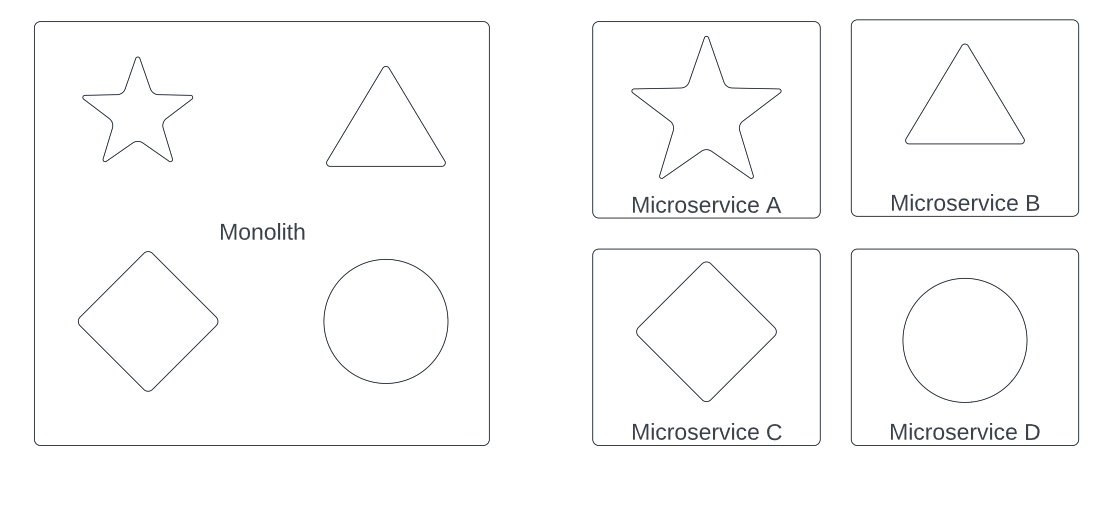
\includegraphics[width=\textwidth]{images/microservices-monolith.png}
	\caption{A very abstract illustration of a monolith and micoservices according to \cite{lewis_microservices_2014}}
	\label{fig:msa}
\end{figure}
%A long list of successful big companies use now MSA (nicht aufzählen).

% zeichnung anlehnen an lewis & fowler

%Bei bedarf nachteile von monoliths nach dragoni et al.

What does distinguish MSA from other architectural styles? It helps to first take a look at the opposite, which would be a monolithic architecture, where the functionality of a system is bunched together and components can not function independently \cite{dragoni_microservices_2017}. MSA on the other hand can be described as a system consisting of a bundle of (micro)services. Each component is now a separate service that can be deployed independently and might even be written in a separate language \cite{lewis_microservices_2014}. They are only loosely coupled \cite{dragoni_microservices_2017} and usually communicate via a RESTful protocol \cite{lewis_microservices_2014}, \cite{dragoni_microservices_2017}, \cite{nehme_securing_2019}. Lewis \& Fowler call this principle "smart endpoints and dumb pipes". A very abstract illustration of the concept of microservices compared to a monolith is shown in figure \ref{fig:msa}.


%Definitionen nach dragoni et al.
%A microservice is a process that can be deployed independently and communicates via messages \cite{lewis_microservices_2014}, \cite{dragoni_microservices_2017}.


Of course MSA comes with certain pros and cons. Advantages of MSA are \cite{dragoni_microservices_2017}:
a) A single microservice consists of a small code base in comparison to a monolith, due to its reduced functionality. It can be tested and debugged independently from the rest of the system. b) When changes are necessary, the microservice in question can be redeployed independently of the rest of the system. c) High flexibility for scaling (instances can be deployed where needed, instead of duplicating the whole system. d) microservices can be written in any language, framework etc. independently of each other. The only constraint is the communication between them.
%API Gateway - having this is a common model according to Nehme et al. \cite{nehme_securing_2019}.% wen erwähnt floren noch? -> evt. abbildung... NIST beschreibt das auch

The same characteristics that bring these advantages also bring certain disadvantages and challenges especially in terms of security. These issues will be reviewed in the next section.

\section{MSA Security Challenges}
\label{sec:security}
Several trust and security challenges arise with MSA. As Dragoni et al. point out, they are not new and already known from Service Oriented Architecture (SOA) and distributed systems, but they gain a new level of impact with MSA \cite{dragoni_microservices_2017}. The issues identified are as follows:
\begin{itemize}
\item \textbf{Large surface attack area}: With the fact that microservices are deployed independently (which is one of the biggest strengths of MSA) comes one of the biggest security challenges that arise with MSA: a high number of endpoints exposed to the network, which creates a much larger surface attack area than a monolithic architecture would normally do, where communication is done internally \cite{dragoni_microservices_2017}, \cite{yarygina_overcoming_2018}, \cite{de_almeida_authentication_2022}%, wer noch? haben das in den findings aber sind nicht die ersten (reicht aber so auch...)
% "Rephrasing, this means that microservices can in principle send the attack surface of a given application through the roof." zitat dragoni et al.
\item \textbf{Network complexity}: Although the single microservice is of an overseeable size and structure, the whole system can become very complex, consisting of a high number of microservices interacting with each other. This can make monitoring, auditing, debugging and forensic analysis even more difficult.
\item \textbf{Trust}: At the time when the work of Dragoni et al. was written, microservices often communicated with each other on a basis of trust. Obviously, this is not an ideal situation and mechanisms are necessary that allow secure communication between microservices in order to minimize the damage that can be done by an attacker that is able to compromise a microservice. %da müsste man jetzt eigentlich schon anmerken, dass das blind trust ein no-go ist aber lästig zum zitieren - ???referenz zu threats section?
\item \textbf{Heterogeneity}: A MSA is heterogeneous by design, since it is composed of different entities, performing a large number of interactions across different administrative security domains and so on.
\end{itemize}

% jetzt schaun, was de almeida und vielleicht auch berardi et al. dazu sagen

%Microservices very popular, examples, Netflix etc....
%Schau auch in den anderen Microservices-Bachelorarbeiten nach, wie weit die da ins Detail gegangen sind. Und natürlich alles, was die großen Surveys dürfen, darf ich schon lang.

%Was ist das überhaupt? Newman als Quelle gut? Zumindest Startpunkt. Was schreiben meine anderen Quellen da?
%Kurze Beschreibung der Architektur, drauf hinleiten, dass das mehr Endpoints bietet. -> Nehme et al?

%Designing a secure MSA means negotiating a tradeoff between security and performance \cite{floren_implementation_2021}, \cite{yang_research_2020}, %\cite{he!!!}!!! zitat verifizieren!.
%Similarly, it is also important to keep in mind that the different security patterns for microservices might compromise some of the characteristics of MSA and as a consequence jeopardize important advantages, e.g. [!!! Beispiele wie Single POint of failure (wo?) scalability, developers focusing on one functionality at a time (Florén -> security patterns).

%Communication in Microservices
%HTTP(S), REST...

%Kurze ankündigung der nächsten kapitel -> api gateway nicht dabei, hier kurz anschneiden?

% evt. threats and risks subsection streichen und das nötigste hier integrieren!
%owasp api threats top 10 erwähnen aber auf keinen fall aufzählen, nur dazusagen, dass einige davon mit authorization und authentication zu tun haben. kann auch in die einleitung zur nächsten subsection.

Berardi et al. \cite{berardi_microservice_2022} also found several other problems in the research area of microservices security. While the research does exist, there are still the following open issues: a) Lack of dedicated attack trees and thread models. b) Technology transfer from academia to industry (lack of tools and methods for validation and verification as well as concrete applications). c) Security-by-design adoption (lack of references or guidelines). d) Lack of comprehensive, concrete references to secure specific technology stacks. It should be noted that this is not a comprehensive list of Berardi et al.'s findings, which go in part beyond the scope of this thesis. The present thesis can not address all of these issues, but it is an attempt to bring more clarity into the microservices security field by taking a closer look at the technology stack that is reported to be in use for authorization and authentication.\\

Unconveniently, there seems to be no generic threat model in use for the security of microservices \cite{berardi_microservice_2022}. Berardi et al. offer as an explanation that the bigger part of the research on microservice security - at least of the literature they have included in their survey - does not come from the field of security research, but from the perspective of software engineering. The OWASP API Security Top 10 lists Broken Object Level Authorization as number 1 risk, followed by Broken User Authentication and Broken Function Level Authorization as number 5 \cite{noauthor_owasp_2019}. Since microservices rely on APIs for communication, these risks are highly relevant for MSA.

%Attacks: lösungen werden in meiner arbeit auch nicht unbedingt behandelt, also eher sein lassen.

%Of course, authorization and authentication is not all one should think about when designing a secure MSA \cite{billawa_sok_2022}, was noch?!!!. Encryption ...

%\subsection{Threats and Risks}
%\label{sec:UnterUnterkapitel21}

%confused deputy? -> Nehme et al. (nr zwei bei florén)
%powerful token theft \cite{nehme_fine-grained_2019}
%Außerdem noch bei den anderen schaun, welche Threats spezifisch nach Authentication and Authorization verlangen.
%OWASP!

%OAuth 2.0 threat model RFC 6819!
\section{Authentication and Authorization in MSA}
\label{sec:msa-authx}
As we have seen in the previous sections, when talking about security in microservices, both, authentication and authorization are considered to be among the most important topics. In this section, a clarification is given how the two concepts differ and what their role is in the context of MSA. % and they are also discussed the most in academic literature (wie isses mit grey lit.?) (Billawa et al.).\\

Authentication and authorization, although they sound very similar, are two distinctive concepts and it is important to understand the difference between the two.
To put it very shortly, authentication is about identity and authorization is about permissions. When someone authenticates, they usually provide a proof of the fact that what they say who they are is true. Identity can be proven with something they know (e.g., a secret password), something they have (like a phone number, to which a code can be sent), or something they are (like biometric data), or a combination of those (e.g. in two-factor authentication where a user gives their username and password, but the authentication is only complete when they also give a code that was sent to their phone number or e-mail address). Not only a person can prove their identity. A system can authenticate as well, for example with a secret or certificate or both. Authorization on the other hand deals with the question what a person or entity is allowed to do, for example where they can enter. Because this usually depends on who they are, in order to determine which permissions someone or something has, authentication is necessary first. Siriwardena \cite[p.~133]{siriwardena_advanced_2020} gives a visa control at a border as example: A person who wants to cross the border has to authenticate - their picture and/or fingerprint might be validated as truly belonging to that person, perhaps also by comparing to a database. This is authentication. Knowing who that person is does not get this person across the border, unless they have a visa. The visa has to be valid and not expired and can contain further details about what you are allowed to do in that country \cite[p.~133]{siriwardena_advanced_2020}.
%siehe auhc chocolate vs. fudge oauth.net/articles/authentication Justin Richer)\\

%vergleich mit monolithic a. -> Nic Jackson auch noch angeben? wegen den tokens warats
Now, what is special about authentication and authorization in a MSA? In a monolithic architecture, when a user wants to access a resource, they authenticate with the system and might get back a session token, which can be sent with every subsequent request to the system. The token can then be validated inside the system, and it will know if this user has the necessary permission for the requested transaction. The same process becomes way more complex in MSA. While a monolithic application only has few entry points, a MSA has at least as many entry points as deployed services and each of them should be protected \cite{jackson_microservice_2019}, \cite{dragoni_microservices_2017}. When a requested resource or service does not sit inside the same system as the service where the user has authenticated themselves, the first service does not know if it can trust whoever made this request without either making another request to the server responsible for dealing with authentication and permissions, or having a way to validate the token locally, without further communication, which might not always be possible. This results in a higher number of requests between services and therefore in potentially decreased performance of the MSA.% \cite{siriwardena_microservices_2020}.\\

To make everything worse, not only access by external end-users has to be managed, but also communication between services. Although the MSA principle demands loosely coupled microservices, it is sometimes inevitable that one service has to talk to another service in order to fulfil its job. But a service should not be reachable by any other microservices in the system, only by those who have a good reason to do so \cite{yarygina_overcoming_2018}. When a service talks to another service on behalf of a user, the user information (authentication and authorization) can be passed on down the line, so each microservice knows who they are working for. This is called principal propagation \cite{yarygina_overcoming_2018}.\\

%third-party access...

%oauth2+oidc hier schon ankündigen?



%\subsection{The API Gateway}
%\label{sec:UnterUnterkapitel22}
%Kommt wahrscheinlich raus, sonst hier anmerken, das das wichtig ist, aber in dieser Arbeit nicht weiter behandelt wird.\\

%While there exist different approaches to the implementation of API Gateways in MSA \cite{floren_implementation_2021}, authors seem to generally agree about the need of at least one API Gateway that stands between the client or end user and the backend microservices.!!!da noch wen zitieren? The beforementioned increased attack surface of an MSA can be reduced dramatically by creating a choke point for all requests  
%\end{comment}

\chapter{Authentication and Authorization Technologies and Standards}
\label{chap:protocols}

In this chapter, the characteristics and parameters of OAuth2, JWT and OIDC will be presented and explained. OAuth2 can be seen as the starting point for this research and JWT and OIDC are closely connected to OAuth2 in the context of authorization and authentication, as will be explained. This chapter aims to give useful information that helps to better understand how they work in general and to explain the importance of certain parameters that will be analyzed in chapter \ref{chap:results}.

%In the following chapter, a collection of standards and protocols commonly used for the purpose of authorization or authentication (or both) will be presented and explained. It should be made clear that this is not a comprehensive list and one might wonder, why Security Assertion Markup Language (SAML) 2.0 RFC!!! is not part of the list. Because the focuses of this thesis lies on implementations of OAuth 2.0, only those technologies that were found to be implemented in combination with OAuth 2.0 in the context of a MSA!!!, or recommended for such an implementation, are listed. It follows that in particular standards that can be used for or are designed for the purpose of authorization are only listed, if they are found to be used or recommended to be used together with OAuth 2.0, like JWT. But, as will be shown later in this work (section xy!!!), SAML, although a popular authentication standard, doesn't seem likely to be used with OAuth 2.0.%!!! nicht mehr aktuell! evt. stattdessen auf de Almeida & Canedo verweisen

\section{OAuth 2.0}
\label{sec:oauth}
% fehlt: OAuth2 beliebt in microservices according to literature, academic + grey! (billawa et al., pereira-vale...)
% genauer drauf eingehen, warum oauth2 für microservices???
% artikel von eran hammer (oauth 2.0 and the road to hell) dazu, um zu illustrieren, wie mühsam es ist + aaron parecki, der sich für das labyrinth entschuldigt (how to hack oauth) -> und trotzdem isses so beliebt.
%ref für industy standard? nate barbettini - redet aber nicht über ms spezifisch
OAuth 2.0, also often referred to as OAuth2, is an open protocol for delegated authorization, defined by the Internet Engineering Task Force (IETF) in the Request for Comments (RFC) 6749 \cite{hardt_oauth_2012} and RFC 6750 \cite{jones_oauth_2012}. Authors of grey and academic literature seem to agree that OAuth2 is the standard for authorization in MSA environment (see chapter \ref{chap:relwork}). OAuth2 was developed to allow a third-party client to access a certain (protected) resource on behalf of the owner of this resource \cite{hardt_oauth_2012}. In a MSA environment, where different services and possibly an API Gateway have to communicate with each other on behalf of a user or of another service, this concept of third-party access makes OAuth2 a feasible solution. The access to a resource happens by means of a so-called \textit{access token}, which is issued to the client from an authorization server and which allows the client, now in possession of this token, to access the protected resource. The token now has to be sent with every request to the server holding that resource.
This chapter gives insight into some of the mechanisms and specifications of the OAuth 2.0 protocol. However, this thesis can not cover all the details of OAuth2 and some concepts have to be described in a simplified manner.

\subsection{OAuth2 Roles}
\label{sec:oauthroles}
% eigener abschnitt über implicit und password grant, warum nicht mehr verwenden???
There are four important roles in the OAuth2 authorization flow \cite{hardt_oauth_2012}:
\begin{itemize}
\item  The \textit{resource owner} is the person or entity that owns a protected resource. The resource owner can grant access to this resource to a third party.
\item The \textit{resource server} is the server where the resource in question lives. It responds to requests containing the access token.
\item The \textit{client} is any application (e.g. a web application or a mobile application) requesting the resource. It is not specified where this application is executed. The client can also act on its own behalf when it is the resource owner at the same time. %public vs. confidential clients steht schon weiter unten, kann aber auch hier noch eingebaut werden.
\item The \textit{authorization server} is the server responsible for authentication of the resource owner, obtaining authorization and issuing access tokens to the client.
\end{itemize}
An example scenario to illustrate these roles would be that a user (the resource owner) has a Facebook account and wants another application (the client) to access data (the protected resource) in their account, maybe because the app has promised to analyze the user's personality based on their timeline posts \cite{jackson_microservice_2019}.\\


\subsection{The OAuth2 Authorization Flow}
\label{sec:oauthflow}

\begin{figure}[htbp]
	\centering
		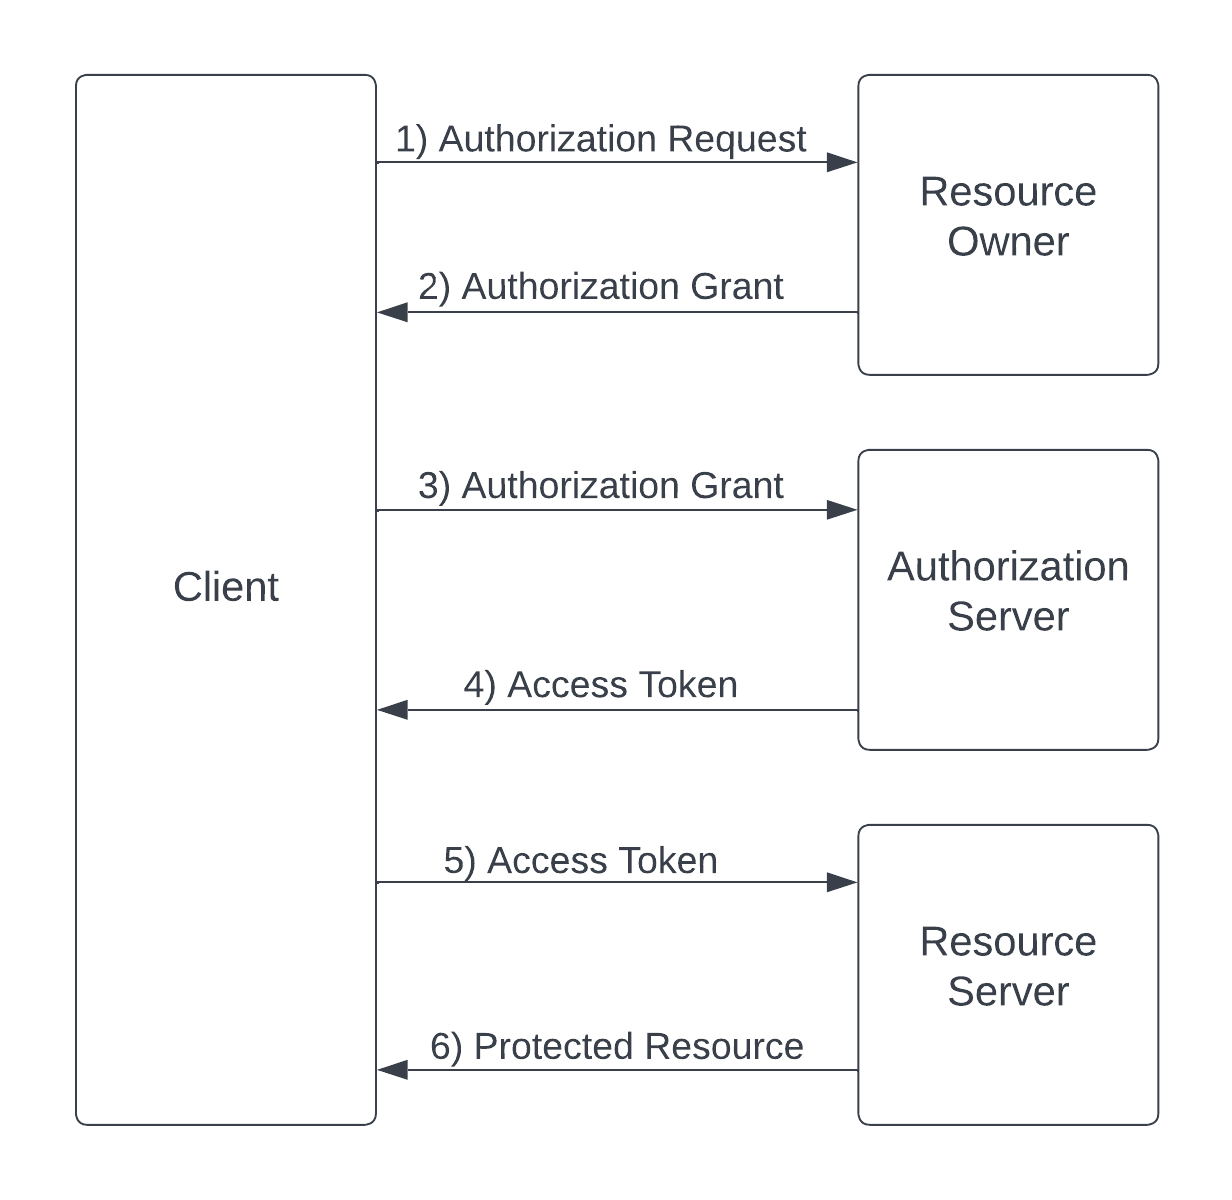
\includegraphics{images/oauth2-flow}
	\caption{Abstraction of the OAuth2 flow after \cite[fig.~1]{hardt_oauth_2012}}
	\label{fig:oauth2flow}
\end{figure}

The simple and most dangerous way for the client to access the user's Facebook data from the example above would be that the user passes their username and password to the client, which can then comfortably log in to the user's Facebook account and do with it whatever it wants to do \cite[p.~81]{siriwardena_advanced_2020}. Obviously, this would lead to many problems if the client, now in possession of the user's credentials, is not trustworthy. OAuth2 solves this problem by enabling the user to grant the client access to their data without letting it see their username and password. This is done by delegating the authorization process to the authorization server. Once the user is authenticated with the authorization server and has given permission to the application to access data from their account, the application will receive the access token and can present this token to the server in exchange for the data they want. The basic steps of the OAuth2 flow are as follows \cite{hardt_oauth_2012} (see also figure \ref{fig:oauth2flow}):%auch auf zeichnung verweisen, sobald die da ist \\
\begin{enumerate}
\item An authorization request is made by the client to the resource owner (preferably via the authorization server)
\item An authorization grant is issued (again preferably via the authorization server) to the client.
\item The client requests an access token from the authorization server by presenting the authorization grant.
\item The access token is issued to the client (after authenticating the client and validating the request).
\item The client presents the access token to the resource server and requests the protected resource.
\item The access token is validated by the resource server (locally or by calling the authorization server) and, if successful, responds with the requested resource. 
\end{enumerate}

In reality the authorization grant, which represents the authorization by the resource owner for the client to access a resource, can come in different shapes. 

\subsection{The OAuth2 Authorization Grant Types}
\label{sec:oauthgrants}
The exact flow in which the client can receive the access token can differ, depending on the \textit{grant type}. The original specification defines four different grant types, but it is also possible to define additional grant types \cite{hardt_oauth_2012}. However, not all of those original grant types are still recommended for implementation according to the OAuth 2.0 Security Best Current Practice (BCP) IETF Internet Draft \cite{lodderstedt_oauth_2022}. %evt. auch noch oauth.net und oauth.com anschaun oder siri
\begin{itemize}
\item With the \textit{authorization code grant}, the authorization server responds to the authorization request (after authenticating the resource owner and obtaining authorization) not with the access token, but with a code, which the resource owner's user-agent (e.g. web-browser) will pass on to the client at the redirection URI \cite{hardt_oauth_2012}. The client can then exchange this code for an access token directly with the authorization server, without exposing the token to the resource owner or potentially anyone else. It is also possible for the authorization server to authenticate the client \cite{hardt_oauth_2012}.
\item The \textit{client credentials} grant: The client receives an access token after authenticating itself to the authorization server with its client credentials (a password or public/private key) \cite{hardt_oauth_2012}.  %With this grant type, no refresh token is issued alongside the access token \cite{siriwardena_advanced_2020}.%??? bessere quelle? nicht in RFC6749 gefunden
\end{itemize}

Legacy grant types \cite{parecki_oauth_granttypes}:
\begin{itemize}
\item The \textit{implicit grant} is similar to the authorization code grant, but here the access token is sent to the client directly instead of sending a code first and the authorization server does not authenticate the client \cite{hardt_oauth_2012}.
\item With the \textit{resource owner password grant}, \texttt{password grant} for short, the resource owner's credentials are directly exchanged for an access token \cite{hardt_oauth_2012}.
\end{itemize}

Other grant types are the \textit{device code} grant, which is an extension \cite{denniss_oauth_2019}, and sometimes also the \textit{refresh token} \cite{hardt_oauth_2012} is called a grant type \cite{parecki_oauth_nodate}, \cite[p.~372]{siriwardena_microservices_2020}, although it is not considered as such in the original OAuth2 specification \cite{hardt_oauth_2012}.

The choice of the grant type depends strongly on the type of the client. The authorization code grant type is optimized for confidential clients, which are capable of keeping their client credentials secret \cite{hardt_oauth_2012}. Public clients, such as web-browser applications or native (mobile) applications, which cannot maintain confidentiality of their secrets were intended to use the implicit grant type in the original specification. The problem with this grant type is that the access token is not issued to the intended client directly, but is handed over by the user-agent, as in \texttt{client.example/redirection\_endpoint\#access\_token=abcdef}, and URLs are often stored in browsing histories \cite{lodderstedt_oauth_2022}. So in order to prevent access token leakage and replay attacks, it is now recommended that public clients should use the authorization code grant as well, with mandatory Proof-Key for Code Exchange (PKCE) \cite{lodderstedt_oauth_2022}. The PKCE, pronounced "pixie", enables clients that are not able to maintain a secret to use the authorizaton grant flow, but it is recommended for all clients \cite{lodderstedt_oauth_2022}. Also the client credentials grant is reserved for confidential clients only \cite{hardt_oauth_2012}, and is used mostly for interaction between systems when no end-user is present, for example a web application accessing an API for metadata \cite[p.~372]{siriwardena_microservices_2020}. In this case, access to the protected resource happens on the client's own behalf.

%??? eigener abschnitt drüber, warum implicit und password grant nicht bennutzt werden sollten?
Although the discussion about whether or not to use certain grant types has gone on for some years already, the OAuth2 BCP, in which the use of the implicit grant is discouraged and the password grant type is dismissed altogether, is rather new: It was first mentioned in version 9 of the OAuth 2.0 BCP in 2018 that "Clients SHOULD NOT use the implicit grant" \cite{lodderstedt_oauth_2018-9} and in version 11 that "The resource owner password credentials grant MUST NOT be used" \cite{lodderstedt_oauth_2018-11}. Therefore, it is important to pay particular attention to the date and origin of tutorials and articles about OAuth2 in order to avoid receiving old information.

%PKCE: must for public clients with auth code grant, recommended for confidential clients, außer conf oidc clients können das irgendwie mit nonce lösen... \cite{lodderstedt_oauth_2022} gibt alle infos dazu!

%???Den folgenden Absatz evt. einfach streichen
%From these options, the Authorization Code grant is presumably the one used the most (sagt wer?!!!). Nevertheless, other grant types are used as well, as the analysis in section (!!!) will show. - neu schreiben, auch password ist nicht mehr cool seit allerspätestens 2019, eigentlich schon früher (quelle?). , while on the other hand it is now strongly discouraged to use the Implicit grant or the Password grant -> oauth best practices.

\subsection{OAuth2 Tokens and Validation}
\label{sec:oauthtoken}
%höher rauf schieben?
%Different types of token !!!
%Aaron Parecki macht key card im hotel vergleich in OAuth: When things go wrong / oder everything you want to know
By some aspects, the access token can be seen as a key to a door \cite{parecki_everything_2021}. It does not contain any information about the person using it, but as long as the key fits, the door will open. But unlike a key, one important security feature with OAuth2 access tokens is that they can expire. To spare the user the effort of having to grant permission again each time the token expires, the client application gets a refresh token along with the access token and once the access token has reached its defined expiration time, the client can then call the authorization server and exchange the refresh token for a new access token. A short expiration time makes it possible to validate access tokens locally, thus reducing the number of necessary calls. In case a permission to a client (represented by the access token) gets revoked at the authorization server, the service will not know this and the access token appears valid with local validation, but only until it expires. Therefore, it is important to evaluate carefully where in the MSA local validation is sufficient and where validation with the authorization server is necessary for higher security \cite{parecki_everything_2021}. In any case, it is highly recommended to never accept unvalidated access tokens \cite{jackson_microservice_2019}.\\
%Hier evt. Zeichnung
\\
%Alle Infos in dem Absatz kommen eigentlich von Siriwardena 2020 (Adv.) -> wo die Referenz hinschreiben?
The nature of the access token is not defined in the OAuth2 specification. It can be an arbitrary string that serves as a reference to the authorization information, or a self-contained token \cite{jones_oauth_2012}. A reference token is susceptible to brute force attacks, therefore additional strategies to prevent brute forcing must be implemented \cite[121]{siriwardena_advanced_2020}. In order to validate a reference token, a call to the issuing authorization server is inevitable. On the other hand, a self-contained token can be validated locally by means of the signature it carries \cite[p.~121]{siriwardena_advanced_2020}. A very popular format for access tokens is the JSON Web Token (JWT) format, which will be discussed in more detail in section \ref{sec:jwt}. In any case, the access token is defined as a string that represents the authorization for the client, but also the scope and duration of access \cite{hardt_oauth_2012}. It has no meaning to the client, similar to how a person does not need to know how a lock and key work in order to open a door.

The definition for access token privilege restriction in RFC 9068 \cite{bertocci_json_oauth_2021} states that access tokens should be restricted to a specific resource server (several resource servers are possible, but preferably only one). This prevents clients as well as users from exceeding their privileges. Resource servers at the other end must check if they are the intended resource server for that access token \cite{lodderstedt_oauth_2022}. The scope is defined by the authorization server. It is not mandatory for a client to ask for a specific scope, but if it does not do that, the authorization server must either fail the request altogether, or issue an access token containing a default scope \cite{hardt_oauth_2012}.

Next to the access token, there is also a \textit{refresh token} \cite{hardt_oauth_2012}. It can be issued to the client together with the access token (with certain grant types) and permits the client to request a new access token when the previous one has expired \cite{hardt_oauth_2012}. With the refresh token it is possible to define short expiration times for access tokens. The new token will not be issued when the permission has been revoked, but as long as this is not the case, the new token can be minted without bothering the resource owner.%!!! quelle nötig? 

%bearer token oder sender-constrained!!!\\

%quasi das gleiche nocheinmal\\
%The specification for OAuth 2.0 [!!! RFC6749] states explicitly that "access tokens can have different formats, structures, and methods of utilization". However, it is very common to use JWT in the OAuth2 flow [!!!RFC9068]. Specifically, in the context of distributed systems like MSA, the use of JWT as access tokens is advisable. One reason is that they can be validated locally and not every single request to the system has to be validated first with the authorization server, which could result in performance loss \cite{yang_research_2020}. They also have the advantage that they usually expire after a while. The drawback of local token validation is that if a token has been revoked, the validating service doesn't know this and will give the client with the token access until it expires [!!! notfalls Nic Jackson]. More details about JWT will be given in section \ref{sec:jwt}. !!!evt. ist das nicht mehr up to date? es gibt sehr frische spec drafts zu oauth.\\


%Security Threats related to Bearer Tokens (!!!RFC 6750) zusammenfassen oder ist das übertrieben?\\
%Trotzdem recommenadations hier? achtung, es gibt ein eigenes rfc mit oauth threat model\\



%oauth.net: access tokens do not convey user information

% was evt noch fehlt: wie ist das mit dem third-party access im kontext von microservices zu verstehen? Wird da irgendwo drauf eingegangen? Siriwardena und Dias: protected resource - client can access, if user authenticates;  client kann first-party acces zu eigenem resource server machen (siehe kommentar oben)



%It is important to note that OAuth2 does not deal with the issue of authentication. Another protocol, OpenID Connect (OIDC), was developed to handle authentication and is build on top of OAuth2. 
%Before OIDC was developed, it was common to use OAuth2 for authentication as well and it still occurred later on, but it is strongly discouraged to do so . More details about OIDC are given in section \ref{sec:oidc}.\\

%bsp hier einfügen, oauth.net artikel zitieren...
\subsection{OAuth2 and Authentication}
Today, when reading about OAuth2, the warning that OAuth2 should not be used for authentication is hard to overlook. Still, authentication is an important component in order to secure a system and OAuth2 can be used \textit{within} an authentication scheme \cite{richer_end_nodate}. With OAuth2, the resource owner will authenticate to the authorization server and also the client has to authenticate to the authorization server in many cases, but it is not the concern of OAuth2 \textit{how} the authentication is done \cite{richer_end_nodate}. In this context it is useful to understand that for the client the access token has no meaning and will just be passed on to the resource server for validation. The client does not learn anything about the user and the fact that an access token was issued should not be misunderstood as a proof that the end-user was correctly authenticated \cite{richer_end_nodate}. When information about the user is needed, OAuth2 is therefore not sufficient to cover authentication, even if this has not been and might still not be an unusual practice \cite{barbettini_oauth_2018}, \cite{jackson_microservice_2019}. The problems and pitfalls associated with the use of OAuth2 for authentication purposes are discussed more in detail in \cite{richer_end_nodate}. Instead, OpenID Connect (OIDC) is a layer on top of the OAuth2 specification and has been developed exactly for this purpose. Details about OIDC are presented in section \ref{sec:oidc}.

%more security aspects: tls - ist MUST in specs, csrf state parameter, nonce (auch in oauth?)

\section{JSON Web Token (JWT)}
\label{sec:jwt}
% evt. als untersection zu OAuth 2.0?
The JSON Web Token format (JWT) is a compact format for transmitting information (also known as claims) between two parties over HTTP and it is defined by the IETF in RFC 7519 \cite{jones_json_2015}. It has become a popular choice for the use as access token in OAuth2, as described in the JSON Web Token (JWT) Profile for OAuth 2.0 Access Tokens specification, RFC 9068 \cite{bertocci_json_oauth_2021}, because it is self-contained and gives the possibility to be validated locally by the resource server (within the limitations discussed in section \ref{sec:oauth}). While it is possible to implement an authorization mechanism using JWTs without the OAuth2 protocol, this topic lies outside the scope of this thesis. The following section will focus on the nature of JWT in general and on its use as OAuth2 access token.

A JWT is a JSON object, encoded in a JSON Web Signature (JWS) or JSON Web Encryption (JWE) structure, or both \cite{jones_json_2015}. This means, it offers the possibility to be cryptographically signed and/or encrypted. Although it is possible to transmit unsigned JWTs, signing JWT access tokens is now mandatory for OAuth2 \cite{bertocci_json_oauth_2021}. Signature algorithms can be either symmetric or asymmetric, but for OAuth2 access tokens, it is recommended to use asymmetric cryptography, and RS256 must be supported by authorization servers as defined in RFC 9068 \cite{bertocci_json_oauth_2021}, but experts have recommended this for some time already, e.g. \cite{jackson_microservice_2019}.

%??? wirklich mind. 2? was ist typisch für OAuth2?
A signed JWT consists of three elements, each of them base64-encoded and separated with a ".". The first element is the JavaScript Object Signing and Encryption (JOSE) header, the second is the JWT payload and the third is the signature \cite{jones_json_2015}. Typically, the JOSE header contains the \texttt{typ}  parameter (defined in the JWT specification \cite{jones_json_2015}, which should have \texttt{JWT} as a value, and, more specifically for OAuth2 access tokens, it must be \texttt{at+jwt} \cite{bertocci_json_oauth_2021}. Special attention will be paid also later in this thesis to the \texttt{alg} parameter, which is not defined in the JWT specification, but in the specification for JWS in RFC 7515 \cite{jones_json_2015-2}. The \texttt{alg} parameter indicates the algorithm used to cryptographically sign the JWT and the respective value must be either registered in the IANA "JSON Web Signature and Encryption Algorithms" registry, or contain a collision-resistant name. As per the RFC 9068, it must never contain "none" as a value. Finally, the \texttt{kid} (key ID) parameter contains a hint about the key that was used to sign the JWS \cite{jones_json_2015-2}. It is optional and can be used to indicate a key change.

The second element of the JWT is the JWT claims set \cite{jones_json_2015}, or JWT payload \cite[p.~160]{siriwardena_advanced_2020}. It contains the "business data" \cite[p.~160]{siriwardena_advanced_2020} of the JWT. The JWT specification does not define which claims are mandatory, but rather leaves this to the specific applications to define. However, it is defined that only claims that are understood by the recipient can be accepted. The JWT specification also defines a list of "registered Claim Names", which are not intended to be mandatory, but are intended as a starting point for further specification. Out of these, the following claims, all defined in RFC 7519 \cite{jones_json_2015}, are required for the use in JWT access tokens \cite{bertocci_json_oauth_2021}:
\begin{itemize}
\item \texttt{iss}: The issuer of the JWT.
\item \texttt{exp}: The expiration time, after which a token must not be processed any more.
\item \texttt{aud}: This parameter identifies the resource for which the access token is intended. It is mandatory as per RFC 9068 in order to prevent cross-JWT confusion, so access tokens issued by the same authorization server for different resources remain unique \cite{bertocci_json_oauth_2021}.
\item \texttt{sub}: The subject of the JWT, either the resource owner (authorization code grant) or the client (client credentials grant), depending on whether a resource owner is involved in granting access \cite{bertocci_json_oauth_2021}.
\item \texttt{iat}: Issuing time of the token. %wörtlich, nur gekürzt von bertocci
\item \texttt{jti}: JWT ID, a unique identifier for the JWT.
\end{itemize}

The kind of access that is requested can be specified within the \texttt{scope} parameter in the request from the client to the authorization server, but often it also contains identifiers for the resource itself or its location \cite{campbell_resource_2020}. To lessen the burden on the \texttt{scope} parameter, there is also a more recent RFC that defines \texttt{resource} \cite{campbell_resource_2020} for the this purpose. However, in the access token, the resource server is indicated not by the \texttt{scope} parameter, but by the \texttt{aud} parameter \cite{bertocci_json_oauth_2021}. Additionally, the \texttt{client\_id} claim, as defined in the RFC 8693 \cite{jones_oauth_2020}, as the name suggests, identifies the OAuth2 client that requested the access token. When using OIDC, other optional claims may become relevant, such as \texttt{auth\_time}, \texttt{acr} and  \texttt{amr}, which are defined in the OpenID Connect Core specification \cite{sakimura_openid_2014}. When first-party clients invoke a backend API belonging to the same solution, it is common that resource owner attributes are carried in the access token.

The access token is issued in response to a request by the client, as in Listing \ref{lst:jwtreq}. The token corresponding to the example request in listing \ref{lst:jwtreq} can be seen in listing \ref{lst:jwtaccess}.


\begin{lstlisting}[frame=lines, caption=Example request for an access token according to \cite{bertocci_json_oauth_2021}, captionpos=b, label = lst:jwtreq, language=C, showstringspaces=false]

   GET /as/authorization.oauth2?response_type=code
           &client_id=2349832dg8s7f87
           &state=123456789
           &scope=%read%write%delete
           &redirect_uri=https%3A%2F%2Fclient%2Eulala%2Enet%2Fcb
           &resource=https%3A%2F%2Frs.ulala.com%2F HTTP/1.1
        Host: authorization-server.ularauch.net
\end{lstlisting}

% nicht-oidc beispiel wäre hier besser, weil oidc noch nicht erklärt wurde. sonst auf oidc-kapitel verweisen.
\begin{lstlisting}[frame=lines, caption=Example JWT access token according to \cite{bertocci_json_oauth_2021}, captionpos=b, label = lst:jwtaccess, language=C, showstringspaces=false]
Header:

      {"typ":"at+JWT","alg":"RS256","kid":"RjEwOwOA"}

   Claims:

{
    "iss": "https://authorization-server.ularauch.net/",
    "iat": "2022-12-31T19:02:23.942Z",
    "exp": "2022-12-31T19:12:23.942Z",
    "aud": "https://rs.ulala.com/",
    "sub": "5ba552d67",
    "jti": "dbe39bf3a3ba4238a513f51d6e1691c4",
    "client_id": "s6BhdRkqt3",
    "scope": "read write delete"
}
\end{lstlisting}

%expiration time - should be short!!! \cite{yarygina_overcoming_2018}
%clock synchronization problem (!!! yarygina), secure token transmission over TLS, private key must kept safe.

%state parameter in oidc - und oauth wahrscheinlich auch... -> doch einen csrf-abschnitt machen? wo am besten?

\section{OpenID Connect (OIDC)}
\label{sec:oidc}
OpenID Connect 1.0 (OIDC) is an open protocol defined as a layer on top of OAuth2 by the OpenID Foundation \cite{sakimura_openid_2014} in 2014. Often there is a need for clients to be able to identify end-users, and OAuth2 does not fulfil this purpose, because it is not intended to be used for authentication. OIDC was developed to close this gap \cite{richer_end_nodate}.

An OIDC flow is very similar to the OAuth2 flow, with a small, but significant difference: in addition to the access token, the authorization server, which is also responsible for handling authentication of the end-user, thus now being an OIDC provider or authentication server, issues also an ID token \cite{sakimura_openid_2014}, \cite{richer_end_nodate}.
The client can also send the access token to the UserInfo Endpoint (at the OIDC provider), which will return a defined set of additional standard claims about the user \cite{sakimura_openid_2014}.
%---Zeichnung für OIDC flow hier---\\
The OIDC flow consists of the following steps \cite{sakimura_openid_2014}:
\begin{enumerate}
\item Authentication request from the client to the OIDC provider
\item Authentication of the end-user at the OIDC provider + obtaining authorization
\item ID token (and usually access token) issued by OIDC provider to client
\item UserInfo request with access token from client to UserInfo endpoint
\item UserInfo response from UserInfo endpoint to client
\end{enumerate}

The OIDC specification provides three specific authentication flows \cite{sakimura_openid_2014}:
\begin{itemize}
\item The \textit{authorization code flow}, similar to the process described for the authorization code grant in section \ref{sec:oauthgrants}, but an ID token is issued to the client together with the access token.
\item The \textit{implicit flow}, again similar to the OAuth2 implicit grant. The OIDC provider redirects the end-user to the client, together with the ID token and the access token.
\item The \textit{hybrid flow} combines characteristics from both other flows. Clients receive always an authorization code and additionally the access token or the ID token. The other token can be exchanged for the authorization code.
\end{itemize}

As per the OAuth2 specification, an access token is opaque to the client \cite{hardt_oauth_2012}. In order to maintain this requirement, the ID token carrying information for user authentication is a separate token, issued alongside the access token \cite{sakimura_openid_2014}. The ID token is a JWT, containing claims similar to the OAuth2 access token, such as \texttt{iss, aud, exp, iat} (see section \ref{sec:oauth}, but also the \texttt{sub} claim, to uniquely identify the subject (end-user) with the client, \texttt{nonce}, which is used to prevent replay attacks and to associate the ID token with a client session, and other optional claims (\texttt{acr, amr, azp}). Other claims are possible as well, however, claims must be understood or be ignored otherwise. An example for an ID token is given in listing \ref{lst:idtoken}, where also the \texttt{auth\_time} claim is used, denoting the time when the user has authenticated. An OIDC authentication request is an OAuth2 authorization request where the \texttt{scope} parameter must be present with \texttt{open\_id} as a value. Other values for \texttt{open\_id} can be present as well \cite{sakimura_openid_2014}.\\

%section 3.1.2.1.
\begin{lstlisting}[frame=lines, caption=Example for an ID token according to \cite{sakimura_openid_2014}, captionpos=b, label = lst:idtoken, language=c, showstringspaces=false]
 {
   "iss": "https://server.ularauch.net",
   "sub": "24400320",
   "aud": "s6BhdRkqt3",
   "nonce": "n-0S6_WzA2Mj",
   "exp": 1311281970,
   "iat": 1311280970,
   "auth_time": 1311280969,
   "acr": "urn:mace:incommon:iap:silver"
  }
\end{lstlisting}

%section 5.3.2
\begin{lstlisting}[frame=lines, caption=UserInfo Response example according to \cite{sakimura_openid_2014}, captionpos=b, label = lst:userinfo, language=c, showstringspaces=false]
  HTTP/1.1 200 OK
  Content-Type: application/json

  {
   "sub": "248289761001",
   "name": "Ula Rauch",
   "given_name": "Ursula",
   "family_name": "Rauch",
   "preferred_username": "ulala",
   "email": "ursula.rauch@stud.fh-campuswien.ac.at",
   "picture": "http://ularauch.net/ulala/ula.jpg"
  }
\end{lstlisting}


Although the ID token appears to be very similar to an access token, there are some important differences to be pointed out \cite{parecki_oauth_nodate}:%https://oauth.net/id-tokens-vs-access-tokens/ - genaue seite angeben?
\begin{itemize}
\item The audience: ID tokens should only be sent to and read by the OAuth2 client. Consequently, ID tokens should never be sent to an API. Access tokens should be read only by the API (the resource server) it was meant for, but never by the client.
\item The format: the format for access tokens is not specified, it can be a JWT, but it can also be an arbitrary string, while on the other hand an ID token is always a JWT.
\end{itemize}

OIDC also defines a protected resource at the OIDC provider, the UserInfo endpoint, where the client can request a set of standard claims with meta-data about the user in question in exchange for the access token \cite{sakimura_openid_2014}. An example for these claims is shown in listing \ref{lst:userinfo}. Also, like in the initial authentication request, the \texttt{scope} parameter must be present with the value \texttt{open\_id} in the request for userInfo claims \cite{sakimura_openid_2014}.

%Ende: betonen, dass das nicht obligatorisch ist? steht bei richer, aber kommt aus der oidc spec nicht so raus.

% Noch mehr OIDC:

%Why - pitfalls with using OAuth2: evt. auslassen, nur das wichtigste funktionale

%Important to not confuse it with OpenID, which is not just a short name of OpenID Connect, but rather the other way round, OpenID is independent of OAuth 2, while OpenID Connect is its extension 

%trennung zwischen access token und id token essentiell -> inhalt vom access token geht den client wenig an, dafür kann mit infos aus id token eine session gemacht werden \cite{ideskog_oauth_nodate} (bis eine bessere quelle kommt, spec lesen!)

\chapter{Methodology}
\label{chap:methodology}
In this chapter the methodology will be described that was used to extract the information presented in chapter \ref{chap:results}.

First, sources were extracted from the works of de Almeida \& Canedo \cite{de_almeida_authentication_2022}, Leines-Vite et al. \cite{leines-vite_information_2021} and Hannousse \& Yahiouche \cite{hannousse_securing_2021}. More precisely, all sources that were referenced in connection with OAuth2, were collected, which resulted in a list of 22 references. Subsequently, these were divided into two groups: publications presenting any kind of implementation as a PoC on the one hand, and publications presenting literature surveys or general recommendations on the other hand. The second group was not used for further analysis, because the sources considered in those publications were already listed separately. The first group then contained 15 sources for further analysis.
%This method limits the research to more recent publications, since literature surveys older than from 2019 were excluded. The oldest publication in the first group is from ...!!!wer? funktioniert nicht wirklich, weil jetzt auch tanh von 2017 und preuveneers & joosen 2017 dabei sind und einige von 2018

Additionally, Google Scholar, IEEE Xplore and ResearchGate were used to search for recent publications, using combinations of "auth", "authentication", "authorization", "security", together with "microservice", "micro-service", "micro service" and the plural. This brought 5 additional recent publications to light, which could be included in the list, on the premise that they mention the implementation of OAuth2.
%???Aufzählen?

The resulting 20 sources were then checked for signs of the implementation of following parameters
\begin{itemize}
\item OAuth2
\item JWT as Access Token
\item OpenID Connect for authentication
\item OAuth2 grant type
\end{itemize}
Signs could be an explicit description, but also code snippets, screenshots or diagrams. Including OAuth2 in this list of criteria seems redundant but this step was necessary, because, as it turned out, some of these sources did mention OAuth2 only as an alternative to their own appproach.\\

%???auch csrf? During the analysis it became apparent that authors sometimes refer to the RBAC or ABAC model, so the implementation of RBAC and ABAC were documented as well.


\chapter{Results and Discussion}
\label{chap:results}

In this chapter, results of the research are presented and discussed. Table \ref{tab:results} gives an overview of the information found in the publications. The subsequent sections discuss the results for the respective parameters. As we can see in table \ref{tab:results}, not all publications contain all the relevant information, but some insights are still possible.

% Please add the following required packages to your document preamble:
% \usepackage{graphicx}
% \usepackage[table,xcdraw]{xcolor}
% If you use beamer only pass "xcolor=table" option, i.e. \documentclass[xcolor=table]{beamer}
% Please add the following required packages to your document preamble:
% \usepackage{graphicx}
% \usepackage[table,xcdraw]{xcolor}
% If you use beamer only pass "xcolor=table" option, i.e. \documentclass[xcolor=table]{beamer}
\begin{table}[]
\resizebox{\textwidth}{!}{%
\begin{tabular}{|l|l|l|l|l|l|}
\hline
\rowcolor[HTML]{FFFFFF} 
\textbf{Reference}                 & \textbf{OAuth}              & \textbf{JWT}                     & \textbf{Signature Algorithm}  & \textbf{OIDC}                       & \textbf{Grant type}                \\ \hline
\cellcolor[HTML]{EDEDED}\cite{chatterjee_applying_2022}  & \cellcolor[HTML]{EDEDED}yes & \cellcolor[HTML]{FFC000}yes      & \cellcolor[HTML]{70AD47}ES256 & \cellcolor[HTML]{FCE4D6}yes         & \cellcolor[HTML]{8EA9DB}AC         \\ \hline
\cellcolor[HTML]{EDEDED}\cite{chatterjee_sftsdh_2022}  & \cellcolor[HTML]{EDEDED}yes & \cellcolor[HTML]{FFC000}yes      & \cellcolor[HTML]{70AD47}ES256 & \cellcolor[HTML]{FCE4D6}yes         & \cellcolor[HTML]{8EA9DB}AC         \\ \hline
\rowcolor[HTML]{FFFFFF} 
\cellcolor[HTML]{EDEDED}\cite{nguyen_bmdd_2022}  & \cellcolor[HTML]{EDEDED}yes &                                  &                               &                                     &                                    \\ \hline
\cellcolor[HTML]{EDEDED}\cite{pasomsup_ht-rbac_2021}  & \cellcolor[HTML]{EDEDED}yes & \cellcolor[HTML]{FFC000}yes      & \cellcolor[HTML]{70AD47}HS256 & \cellcolor[HTML]{FCE4D6}maybe       & \cellcolor[HTML]{FFFFFF}           \\ \hline
\cellcolor[HTML]{EDEDED}\cite{jin_secure_2020}  & \cellcolor[HTML]{EDEDED}yes & \cellcolor[HTML]{FFC000}yes      &                               &                                     &                                    \\ \hline
\cellcolor[HTML]{EDEDED}\cite{yang_research_2020}  & \cellcolor[HTML]{EDEDED}yes & \cellcolor[HTML]{FFC000}yes      & \cellcolor[HTML]{70AD47}RSA   & \cellcolor[HTML]{FFFFFF}            & \cellcolor[HTML]{8EA9DB}AC + PW    \\ \hline
\cellcolor[HTML]{EDEDED}\cite{baker_novel_2020}  & \cellcolor[HTML]{EDEDED}yes & \cellcolor[HTML]{FFC000}yes      &                               & \cellcolor[HTML]{FFFFFF}            & \cellcolor[HTML]{8EA9DB}AC+CC+I+PW \\ \hline
\rowcolor[HTML]{FFFFFF} 
\cellcolor[HTML]{EDEDED}\cite{kramer_implementing_2019}  & \cellcolor[HTML]{EDEDED}yes &                                  &                               &                                     &                                    \\ \hline
\cellcolor[HTML]{EDEDED}\cite{nehme_fine-grained_2019}  & \cellcolor[HTML]{EDEDED}yes & \cellcolor[HTML]{FFFFFF}      & \cellcolor[HTML]{FFFFFF}      & \cellcolor[HTML]{FCE4D6}yes         &                                    \\ \hline
\cellcolor[HTML]{EDEDED}\cite{nguyen_applying_2019} & \cellcolor[HTML]{EDEDED}yes &                                  & \cellcolor[HTML]{FFFFFF}      & \cellcolor[HTML]{FFFFFF}            & \cellcolor[HTML]{8EA9DB}AC         \\ \hline
\cellcolor[HTML]{EDEDED}\cite{preuveneers_towards_2019} & \cellcolor[HTML]{EDEDED}yes & \cellcolor[HTML]{FFC000}yes      & \cellcolor[HTML]{FFFFFF}      & \cellcolor[HTML]{FCE4D6}yes         & \cellcolor[HTML]{8EA9DB}PW         \\ \hline
\cellcolor[HTML]{EDEDED}\cite{triartono_implementation_2019} & \cellcolor[HTML]{EDEDED}yes &                                  & \cellcolor[HTML]{FFFFFF}      &                                     & \cellcolor[HTML]{8EA9DB}PW         \\ \hline
\rowcolor[HTML]{FFFFFF} 
\cite{xu_microservice_2019}                         & no                          &                                  &                               &                                     &                                    \\ \hline
\rowcolor[HTML]{FFFFFF} 
\cite{yarygina_overcoming_2018}                         & no                          &                                  &                               &                                     &                                    \\ \hline
\cellcolor[HTML]{EDEDED}\cite{banati_authentication_2018} & \cellcolor[HTML]{EDEDED}yes & \cellcolor[HTML]{FFC000}yes      & \cellcolor[HTML]{FFFFFF}      & \cellcolor[HTML]{FCE4D6}no (OpenID) & \cellcolor[HTML]{8EA9DB}AC         \\ \hline
\cellcolor[HTML]{EDEDED}\cite{guija_identity_2018} & \cellcolor[HTML]{EDEDED}yes & \cellcolor[HTML]{FFC000}yes      & \cellcolor[HTML]{FFFFFF}      & \cellcolor[HTML]{FCE4D6}yes         & \cellcolor[HTML]{8EA9DB}PW + CC    \\ \hline
\rowcolor[HTML]{FFFFFF} 
\cite{jander_defense--depth_2018}                         & no                          &                                  &                               &                                     &                                    \\ \hline
\rowcolor[HTML]{FFFFFF} 
\cite{lu_secure_2017}                         & no                          &                                  &                               &                                     &                                    \\ \hline
\cellcolor[HTML]{FFFFFF}\cite{preuveneers_access_2017} & \cellcolor[HTML]{FFFFFF}no  &                                  &                               &                                     &                                    \\ \hline
\rowcolor[HTML]{FFFFFF} 
\cellcolor[HTML]{EDEDED}\cite{thanh_embedding_2016} & \cellcolor[HTML]{EDEDED}yes &                                  &                               &                                     &                                    \\ \hline
\end{tabular}%
}
\caption{Results of the analysis. Signature algorithms: ES256 - ECDSA SHA256, HS256 - HMAC SHA256; Grant types: AC - authorization code, CC - client credentials, I - implicit, PW - password.}
\label{tab:results}
\end{table}

The earlier publication of Preuveneers \& Joosen \cite{preuveneers_access_2017}, originally included in the set of publications for further analysis because it has been listed by de Almeida \& Canedo \cite{de_almeida_authentication_2022} in the context of OAuth2, turned out to mention OAuth2 but not because they had actually included it in their implementation. They state that scope, as it is used by OAuth2 to distinguish different access levels, is not rich enough for a more fine-grained access control policy, as provided by the Extensible Access Control Markup Language (XACML). They also propose the possibility of combining both, but this is is merely a side mark in their work, which is focused mainly on their own, XACML-inspired ACAB policy language.

Similarly, Yarygina \& Bagge \cite{yarygina_overcoming_2018}, Xu et al. \cite{xu_microservice_2019}, Jander et al. \cite{jander_defense--depth_2018} as well as Lu et al. \cite{lu_secure_2017}, all referenced by de Almeida \& Canedo \cite{de_almeida_authentication_2022}, do mention OAuth2 as a possible solution in their work, but in their implementations they choose different approaches.

In the end, of 27 sources collected at the beginning, only 15 mention the actual implementation of OAuth2. Unfortunately, they do not always give much detail about their chosen approach and configuration.

\section{JWT as Access Token}
\label{sec:res-jwt}
The first parameter to be analyzed is the use of JWT as OAuth2 access tokens. The OAuth2 specification leaves explicitly open what format or structure the access token should have \cite{hardt_oauth_2012}. Although the JWT format is just one option, it is reportedly considered the industry standard for OAuth2 access tokens \cite{preuveneers_towards_2019}. Nevertheless it has not become completely clear in previous literature surveys how often and in which of their sources this is actually the case.
Of the 15 examined sources with an OAuth2 implementation, 9 report the use of JWT as access tokens \cite{yang_research_2020}, \cite{jin_secure_2020}, \cite{banati_authentication_2018}, \cite{guija_identity_2018}, \cite{chatterjee_applying_2022}, \cite{chatterjee_sftsdh_2022}, \cite{baker_novel_2020}, \cite{pasomsup_ht-rbac_2021}, \cite{preuveneers_towards_2019}.

Yang \& Hu \cite{yang_research_2020} motivate their choice for JWT tokens as follows: 1) JWTs can be digitally signed and therefore verified locally without the need to contact an authorization server every time. 2) JWTs can carry information about the user. The second point confirms the common concern that OAuth2 deals with authorization only and that it should not be used for authentication. This leads to the question whether OpenID Connect is implemented for authentication, which is not the case here. This issue is discussed further in section \ref{sec:res-oidc}.

Although they do not mention JWT explicitly, it can be assumed that Nehme et al. \cite{nehme_fine-grained_2019} use JWT tokens as well, because they describe the use of OIDC which relies on JWT. It is unlikely that JWT is used for ID tokens but not for access tokens.

We can see clearly that JWT is a popular format for OAuth2 access tokens in MSA with one half of the sources describing its use explicitly. It is also possible that the percentage is actually much higher, because where JWT was not mentioned, information about the format of the access token was not present at all and alternatives to the JWT format could not be found in this context.
\section{Algorithm Choice for Signing JWT Tokens}
\label{sec:res-alg}
Another important detail is the algorithm choice for signing the JWT. This can be done either by using a symmetric algorithm (with a shared secret) or with an asymmetric algorithm (public and private key - see section \ref{sec:jwt}. Of the 9 sources with JWT access tokens, only four mention the cryptographic algorithm in some way.

Yang \& Hu \cite{yang_research_2020} present a model for unified authentication and authorization in MSA, based on OAuth2, including the command to be used in order to generate a public-private RSA key pair for JWT signatures. They still mention both options, symmetric (HMAC) or asymmetric (RSA or ECDSA) keys, in their introduction.

Contrary to most other publications, Chatterjee \& Prinz \cite{chatterjee_applying_2022} and Chatterjee et al. \cite{chatterjee_sftsdh_2022} mention explicitly the use of SHA256 with ECDSA (ES256) for JWT signatures. In both papers, solutions are presented to secure personal health data in an Internet of Medical Things (IoMT) environment. Chatterjee \& Prinz \cite{chatterjee_applying_2022} have developed a prototype electronic health coachin (eCoach) system using Spring Security Framework and Keycloak, an open source identity and access management (IAM) tool with implemented OAuth2 for open authorization, multi-factor authentication, identity brokering, and user management. Chatterjee et al. \cite{chatterjee_sftsdh_2022} also present an eCoach prototype but instead of Keycloak, this time they use Services for Sensitive Data (TSD)\footnote{\label{tsd}https://www.uio.no/english/services/it/research/sensitive-data/}.
%They also give detailed information about CSRF prevention \cite{chatterjee_sftsdh_2022}, which is beyond the scope of this thesis but still worth mentioning.

Pasomsup \& Limpiyakorn \cite{pasomsup_ht-rbac_2021} describe the JWT format and its benefits in the background section before introducing their own prototype that integrates OAuth2 for role-based access control (RBAC). In this general description, the symmetric HMAC SHA256 (HS256) algorithm is mentioned as the "cryptographic algorithm normally used". They also show an example JWT with HS256 as value for the \texttt{alg} header parameter. However, they do not talk about signature algorithms in the part about the prototype.

What we can learn from this is first of all that this parameter is not considered important enough to be explicitly mentioned by most authors, with the noteworthy exception of Chatterjee \& Prinz \cite{chatterjee_applying_2022} and Chatterjee et al. \cite{chatterjee_sftsdh_2022}. Also, we can not assume that asymmetric algorithms, even if used by a majority in this very small set of occurences, are the default choice for all authors, since HS256 was described as the "normal" choice by Pasomsup \& Limpiyakorn \cite{pasomsup_ht-rbac_2021}.
\section{Authorization Grant Type}
\label{sec:res-grant}
In the OAuth2 authorization process, four grant types were originally introduced, but the \textit{resource owner password grant} has since been dismissed for security reasons and also the use of the \textit{implicit grant} is strongly discouraged in most cases and the \textit{authorization code} grant should be used instead with additional security measurements like PKCE (see section \ref{sec:oauthgrants}).

9 of the analyzed sources contain information about the chosen grant type. Of those who do, three talk only about using the authorization code grant \cite{banati_authentication_2018}, \cite{chatterjee_applying_2022}, \cite{chatterjee_sftsdh_2022}, two mention only the password grant \cite{triartono_implementation_2019}, \cite{preuveneers_towards_2019}, at least one has an authorization server that supports all four original grant types, depending on the type of client \cite{baker_novel_2020}. Yang \& Hu \cite{yang_research_2020}, although they do not talk about grant types, show a piece of configuration code where password and authorization code type are enabled. Similarly, Nguyen \& Baker \cite{nguyen_applying_2019} list the \textit{AuthorizationcodeServices} Interface from the Spring Security Framework in their PoC Development section. This can be taken as a hint that the authorization code grant was used, but it is not enough information to draw any more conclusions. Preuveneers \& Joosen \cite{preuveneers_towards_2019} comment that they use the password grant in their prototype "for simplicity". Finally, Guija \& Siddiqui \cite{guija_identity_2018} use a somewhat unclear terminology, where they talk of the "User Credentials grant type" and "Resource Owner Password Credentials grants" for user accounts. Since no mention of the definition of new grant types is made, it can be assumed that the (resource owner) password grant type is in use. For other microservices and a special \textit{Adapter} component, a client that communicates with the Keycloak server, where the access tokens are issued, the Client Credentials grant type is used. The Adapter has extended authorization functionalities. Together they form the \textit{User Management} module.

\section{OIDC for Authentication}
\label{sec:res-oidc}
It has been explained previously that authentication and authorization are related and occur closely to each other, but they are still two different concepts. It has also been pointed out that OIDC is intended to be used for authentication purposes when OAuth2 is implemented (see sections \ref{sec:oauth} and \ref{sec:oidc}). OIDC was developed after OAuth2, but it comes as a surprise that even in a publication from 2021 \cite{pasomsup_ht-rbac_2021} or 2022 \cite{nguyen_bmdd_2022} OIDC is not even mentioned as the state of the art when a different approach has been chosen.

Publications reporting the use of OIDC for authentication are those of Nehme et al. \cite{nehme_fine-grained_2019}, Guija \& Siddiqui \cite{guija_identity_2018}, Chatterjee \& Prinz \cite{chatterjee_applying_2022}, Chatterjee et al. \cite{chatterjee_sftsdh_2022} and Preuveneers \& Joosen \cite{preuveneers_towards_2019}, which means only five sources in total.

Guija \& Siddiqui \cite{guija_identity_2018} present an authentication and authorization solution in a 5G platform for services virtualization, orchestration and management. Like Chatterjee \& Prinz \cite{chatterjee_applying_2022}, they use Keycloak with OAuth2, OIDC and JWT access tokens. They also mention the use of the OIDC hybrid flow for authentication. 

Bánáti et al. \cite{banati_authentication_2018} present an "Authorization and Authentication Orchestrator (AAO)" to manage a system using OAuth2, OpenID, JWT and SSO (which is outside the scope of this thesis). They mention OpenID several times, but not OpenID Connect. They give no source, nor do they describe OpenID as being defined as a layer on top of OAuth2, as usual. Instead they describe it as a method from 2005 that allows users to use the same credentials for different applications. This suggests that they do indeed talk about OpenID and not OpenID Connect as could be assumed with OAuth2.

While OIDC is younger than OAuth2, this does not explain this suprisingly low number of implementations of OIDC. It is possible that OIDC is sometimes seen as a part of OAuth2 and therefore not mentioned explicitly. The work of Pasumsup \& Limpiyakorn \cite{pasomsup_ht-rbac_2021} is not counted with the other four, but they seem to accidently reference OIDC for OAuth2, which might be a hint that OIDC was in place.

%Nicht verwenden, passt hier nicht.
%A special case might be the work of Nguyen et al. \cite{nguyen_bmdd_2022}, who have implemented a broker-less decentralized platform for IoT with decentralized authentication with Decentralized Identity (DID). They compare this approach to centralized authentication with a Aperion CAS server for SSO together with OAuth2. Because their work is focused mainly on the decentralized model, they do not go into detail about the implementation of OAuth2 and no details are given about grant type or any of the other parameters in the aim of this research. However, the findings in their work is noteworthy, because they show how OAuth2 authorization and a centralized identity management might not be the best solution for IoT. Their motivation for finding an alternative is to avoid a single point of failure on the one hand, but on the other hand they also found that in the process for requesting a token and resolving (validating) a token, DID performed much better in terms of highest number of concurrent users, throughput and error.
%nehme et al. noch vorstellen?

%Pasomsup + Limp - machen session mti extra jwt tokens aber erwähnen oidc nicht? checken


%\section{Countermeasures against Cross Site Request Forgery (CSRF}
%\label{sec:res-csrf}
%One very specific concern with OAuth2 is the mitigation of CSRF attacks, where an attacker redirects the client to a different URI than the original callback URI \cite{lodderstedt_oauth_2022}, \cite{chatterjee_sftsdh_2022}. Countermeasures against this type of attack are recommended in \cite{lodderstedt_oauth_2022}: 


%\section{Authentication and Authorization in IoT}
%\label{sec:res-iot}
%


\chapter{Conclusion and Future Work}
\label{chap:conclusion}

In this research it has been shown that with few exceptions, little attention has been paid so far in academic literature in the MSA context to widely discussed parameters of OAuth2, like the choice of authorization grant and the use of OIDC for authentication instead of "misusing OAuth2", as Nate Barbettini puts it \cite{barbettini_oauth_2018}. Because most works focus on different research questions, almost none of the reviewed sources describe explicitly all the parameters that were investigated in this research and many do not mention them at all. But it could be shown that one half of the reviewed sources use JWT as access tokens, only four of them mention the use of OIDC for authentication and neither symmetric algorithms for JWT signatures nor the password grant type are dead in academic literature. On the other hand, in those publications where more details on security parameters were given, the chosen grant type and algorithm were usually compliant to the OAuth2 Security BCP and OIDC was in place as well. But these remain an exception and in the majority of the cases the focus was on different issues entirely.

Limitations to the validity of the outcome of this research are posed by a possible degree of variance or imprecision in the terminology used by authors. For example, authors might be referring to OAuth, having actually the current specification of OAuth 2.0 in mind, but they do not see the necessity to specify the version, because earlier versions are deprecated anyways. It also occured that authors described the use of OpenID Connect without the mention of OAuth(2), but since OpenID Connect lives on top of OAuth2 it can be assumed that OAuth2 was implemented. In the same way, it might be possible that OpenID Connect was implemented but not described explicitly, because it is seen as a part of OAuth2.

Therefore, it is difficult to make absolute statements about the presence or absence of a protocol.

This thesis does not provide new recommendations for the use of OAuth2, except for the conclusion that it would be wise when writing about an implementation of OAuth2 and OIDC to also give details about the parameters mentioned before, but also to explain certain choices because each published example might serve as a model for other researchers. Other than that it can rather be seen as an addition to existing literature surveys, as it gives not only an overview on a range of recent publications as well as such publications from the past years that are frequently referenced, but it also gives more details than more general literature surveys can do, by applying a more narrow scope. It also shows that technology change in the software field can sometimes be very fast and how important it is not only in the industry, but also for academia to keep pace and not hang on to old practices.

There are of course a couple of related topics that this research does not cover. First of all, more detailed information from a security point of view could be given on the type of attacks OAuth2 is vulnerable to in the context of MSA. This could probably be a whole new thesis. It might also be interesting to take a closer look at those sources that got less attention in this research because either they do not describe any implementation of OAuth2, or they do not contain any details about it. What might also be missing is a comparison with other literature on OAuth2, without the limitation on MSA. Also an extension of the survey on grey literature could be worth while, with specific attention to the date, in order to determine if recommendations for the implicit grant type or the use of OAuth2 for authentication come only from older sources. Apart from narrowing the scope to MSA, no distinction has been made between different architectural patterns. A recurrent topic in literature about MSA security is the role of the API gateway (see for example Florén \cite{floren_implementation_2021}) and it could be interesting to analyze sources for different patterns. Also some authors have conducted performance and security testing but the outcomes have been ignored in this thesis because their research questions are beyond its scope. Of course, since the number of practical implementations of OAuth2 in MSA in academic literature is still quite small, a contribution could be made by proposing a model implementation or by further testing of security and performance parameters. This would especially be interesting with alternatives to JWT, like PASETO (cfr. Billawa et al. \cite{billawa_sok_2022}).

It remains to say that the field of OAuth2 is more complex than one would think at first glance and a bachelor's thesis is too small to capture all its details. There are in fact so many RFCs involved that the members of the OAuth Working group themselves started to make jokes about it. Aaron Parecki lists 9 RFCs which are required to be read before implementing a secure solution with OAuth2 \cite{parecki_its_2019} (and he isn't joking there) and Lee McGovern wrote an Article with the title \textit{"OAuth 2.1: How Many RFCs Does it Take to Change a Lightbulb?"} \cite{mcgovern_oauth_2019}, which is good news, because OAuth 2.1 \cite{hardt_oauth_2022} is on its way.

%Conclusion s.o. + es könnte noch sehr viel mehr ausprobiert und nicht nur repliziert werden, außerdem wäre eine genauere Beschreibung und Begründung für die Wahl der jeweiligen Standards und Details in deren Implementierung sinnvoll hilfreich für nachfolgende Forschende und Surveys sollten die Natur der referenzierten Quellen (Survey oder Präsentation von PoC) genauer unterscheiden, um einen Echokammereffekt zu vermeiden (dass das ein Echokammereffekt ist, würde ich an der Stelle einfach behaupten, hab aber keine Referenzen).

%important to follow up-to-date guides and instructions (check date of online-tutorials and rather follow advice from OAuth2 Community o.ä.), check for newer specifications or drafts. oauth2.net und .com sind gute seiten.


%Ausblick, was man sonst noch machen könnte, wenn man viel Zeit hat:


%Was alles nicht: architektur nicht - daher auch nicht mtls - eigenes thema. hätte schon was hergegeben aber hätte dann mehr auf architektur eingehen müssen - ist ok, kommt in die conclusion
%andere standards nicht wie saml2, sso - überlappt sich zwar mit oauth, aber ist 
%irgendwo erklären, warum diese parameter?
%eingeschränkt um dem rahmen der arbeit gerecht zu werden

%Graue Literatur systematischer in die Analyse mit einbeziehen, weil tw. aktueller, evt. auch Tutorials. -> könnte die Lücken besser füllen, die hier offen geblieben sind
%Architekturen anschaun  (wurde hier nicht berücksichtigt, die oben erwähnte MA geht in die Richtung)
%Und noch wichtiger: Use case analysieren, Rollenverteilung -> z.B. macht OIDC oder ein anderer grant type hier überhaupt sinn?
%Alternativen zu JWT als Access Token suchen und vergleichen
%Alternativen zu OAuth2 suchen und vergleichen (Nehme et al. \cite{nehme_securing_2019} criticize the potentially large amount of invalid token requests and load of tokens that need to be stored securely)
%Performance- und/oder Securitytests machen
%Take container technologies into account (siehe florén?)

%difficulties encountered: starting point was already higly specialized literature, sometimes unclear terminology, lack of distinction and detail in literature surveys help of grey literature sometimes false friend, huge number of specifications and "older" grey literature sources describing "best practice" that is not state of the art anymore
%Traurig, dass so viele andere details ausgeblendet werden müssen, die bemerkenswert wären.

%Auch wichtig, nur nicht thema der Arbeit: Principle of least privilege, RBAC/ACAB, secure connections, encryption ...

%\newpage
%\chapter{Future work}
%\label{chap:future}
%generic MSA Threat model (siehe berardi et al.)
%Expand the research to grey literature
%Compare findings to state of the art for monolythic systems, bzw. look for possible solutions without the %limitation of the MSA context and check for applicability in a MSA environment
%by taking away the restriction adopted in this thesis, research on newest developments and propositions that include alternatives to OAuth2 (Nguyen et al 2022)

\newpage
% --- Bibliography ------------------------------------------------------

%IEEE Citation [1]
\bibliographystyle{IEEEtran}
%for alphanumeric citation eg.: [ABC19]
%\bibliographystyle{alpha}

% List references I definitely want in the bibliography,
% regardless of whether or not I cite them in the thesis.

\newpage
\addcontentsline{toc}{chapter}{Bibliography}
\bibliography{bibtextest}

\newpage

% --- List of Figures ----------------------------------------------------

\addcontentsline{toc}{chapter}{List of Figures}
\listoffigures


% --- List of Tables -----------------------------------------------------

\newpage
\addcontentsline{toc}{chapter}{List of Tables}
\listoftables

\end{document}
